% Tento soubor nahraďte vlastním souborem s obsahem práce.
%=========================================================================
% Autoři: Michal Bidlo, Bohuslav Křena, Jaroslav Dytrych, Petr Veigend a Adam Herout 2019

% Pro kompilaci po částech (viz projekt.tex), nutno odkomentovat a upravit
%\documentclass[../projekt.tex]{subfiles}
%\begin{document}

\chapter{Úvod}

Se stále rostoucí závislostí dnešní společnosti na internetu a počítačích se z těchto technologií stala neodmyslitelná součást našich životů. 
Ovšem stále častěji jsou tyto technologie zneužívány útočníky, kteří přicházejí stále s novými metodami, jak napadnou počítače uživatelů a narušit tak jejich soukromý a nebo odcizit citlivé informace.
Proto je nutné, aby prostředky pro boj s těmito útoky byly neustále modernizovány a byly co nejúčinější.

Proto programy pro detekci škodlivého program (z anglického malicious software, dále pak už jen zkráceně malware) založené na strojovém učení, které jsou v současné době využívány, vyžadují vhodnou datovou sadu na které se bude model učit a ověřovat svoji validitu.
Cílem této práce tedy je vytvoření vhodného nástroje na tvorbu datových sad, které jsou nezbytné pro tyto metody. %detekce založené na strojovém učení.
A dále je pak porovnání těchto metod a jejich úspěšnosti při detekci škodlivého softwaru.

Hlavním důvodem, proč se zabývat rozpoznáváním jednotlivých druhů malwaru a jejich klasifikací, je jeho nezbytnost a důležitost.
Jelikož je velice nereálné, že by v následujícíh letech vymizela potřeba se před těmito útoky branít. Ba naopak lze předpokládat, že 
bude příbývat stále více nových druhů škodlivého softwaru, a proto je nutné na tyto změny rychle a efektivně reagovat, aby byla zajištěna
bezpečnost uživatelů internetových sítí.

Tato bakalářská práce se skláda ze 4 kapitol. Toho úvodu, který slouží jako nahlédnutí do problematiky, následují dvě samostatné kapitoly a závěru. V kapitola \ref{2.chap} se nejprve seznámíte s dělení škodlivého softwaru do rodin. Následně
je představeno několik současných řešení detekce škodlivého softwaru, které jsou založeny na strojovém učení a jejich údajná přesnost.
V kapitole s číslem \ref{3.chap} je pak přiblížen způsob jakým byly vytvořeny vhodné datové sady a popis vytvořeného nástroje sloužícího k tomuto účelu. V závěru jsou pak zhodnoceny dosavadní výsledky a postup další práce.

\chapter{Malware a způsoby jeho detekce} \label{2.chap}
%Prejmenovat tuto kapitolu
%Cca 5 stranky co to vůbec malware je a jak se deli a jaké způsoby na detekci se v současné době používají.
%Příklady rodin a nějaké statistiky. Co je statická a dynamická analýza

Tato kapitola se zabývá základy, co je to vůbec malware, jaké jsou jeho typy a jak lze malware dělit. Jak a na základě jakých kritérií lze malware klasifikovat.
Nakonec se zaměřuje na to, jak lze malware analyzovat a na rozddíly mezi statickou a dynamickou analýzou. 


\section{Malware}
Malware (česky škodlivý program) je akronym pro anglický výraz \textit{\textbf{mal}icious soft\textbf{ware}}. Jako malware se označuje jakýkoliv počítačový program nebo binární kód, který provádí jistou 
špatnou činnost a jeho cílem je infikovat počítač uživatele a způsobit mu škodu různými způsoby \cite{malware_book}. %cite https://www.kaspersky.com/resource-center/preemptive-safety/what-is-malware-and-how-to-protect-against-it
                                                                                                % cite the book
Nejpřesnější mi však přijde definice, která říká, že malware je vlsatně kód běžící v počítačovém systému, o jehož přítomnosti nebo chování správci systému vůbec nevědí, protože kdyby o kódu a jeho chování věděli, nedovolili by jeho spuštění.
Malware totiž ohrožuje důvěrnost, integritu nebo dostupnost systému tím, že využívá již existujících zranitelností systému nebo vytváří zranitelnosti nové \cite{article_malware}.%cite https://dl.acm.org/doi/pdf/10.1145/3329786

Často také dochází k záměně a pojmů mezi virem a malwarem. Rozdíl spočívá v tom, že malware je souhrnný termín pro celou řadu hrozem a malware je slovo nadřazené virům. Počítačový virus je jednoduše jedním z typů malwaru.

\section{Klasifikace malwaru}
Jak lze na obrázku \ref{classific} vidět, malware lze klasifikovat na základě různých aspektů. Buď je možné jej rozdělovat podle typu, což je nejčastější způsob, se kterým se v dnešní době lze setkat. Nebo je možné 
jej dělit na základě jeho chování nebo v určité malé míře se lze setkat s klasifikací na základě práv, které malware má v době jeho spuštění \cite{article_malware}. Ovšem s tímhle dělením se zde dále nebudeme zajímat a je zde zmíněno jen pro zajímavost.

\begin{figure}[h]
	\centering
        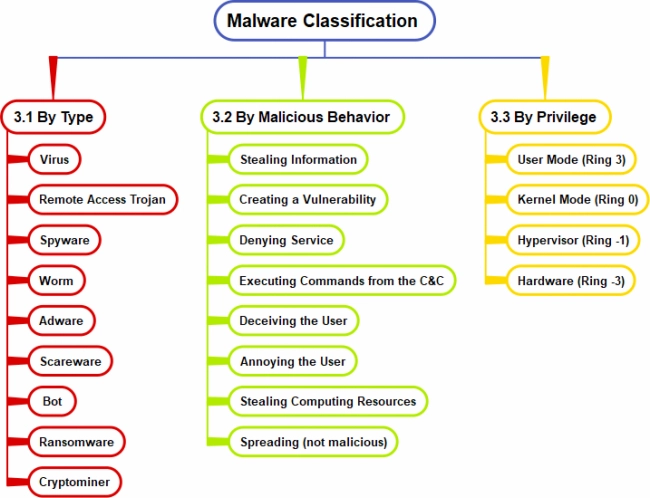
\includegraphics[width=0.7\textwidth]{obrazky/classification.png}
	\caption{Možnosti klasifikace malwaru na základě různých kritérií. Převzato z \cite{article_malware}.}
    \label{classific}
\end{figure}
\newpage
\subsection*{Klasifikace na základě typu}
Jedná se o nejběžnější formu klasifikace, kterou lze kdekoliv najít. Takto lze klasifikovat malware do několika různých skupin. Počet těchto skupin se může nepatrně lišit, protože není pevně daný, ale ve své podstatě jde 
pouze o rozdělení jednoho typu na dva menší podtypy. 

U každého typu je uveden jeho jednoduchý popis a zástupce malwaru, který do tohoto typu patří. Typy malware jsou tedy následující:\cite{kaspersky,article_malware,malware_book,malware_wiki} %cite kaspersky, the paper, and the book, and wikipedia
\begin{itemize}
    \item \textbf{Virus}je program obvykle ukrytý v jiné aplikaci a spustí se, když je aplikace puštěna. Virus se pak může dále šířit pomocí nějakého média, nebo také krást citlivá data. Příkladem virů můžou být například \textit{DarkComet, Stuxnet} \cite{malware_types}. 
    \item \textbf{Trojský kůň} (v angličtině \textit{Trojan horse} nebo pouze \textit{trojan}) je program, který se vydává za normalní program a tím přinutil uživatele k jeho spuštění. Trojský kůň poté lze využít ze vzdáleného počítače nebo serveru jako přístup k uživatelskému počítači a napáchat tak další škody. Příkladem trojského koně je třeba \textit{TrickBot}.  
    \item \textbf{Spyware} je typ malwaru, který monitoruje aktivitu uživatele bez jeho vědomí a tyto informace pak předává útočníkovi. Spyware sleduje uživatelem navštěvované stránky, zeměpisnou polohu a mnoho dalšího. Spyware zaznamenává aktivitu jak online tak offline. Mezi spyware patří například \textit{Gator}.
    \item \textbf{Červ}, ale spíše známý pod svým anglickým jménem tedy \textit{worm}, je spolu s virem nejběžnějším typem malwaru. Je viru velice podobný, ale narozdíl od viru se šíří prostředníctvím počítačové sítě. Jedná se o program, který se neustále replikuje a dále šíří a zatížit tak síť a tím zamezit jejímu používání. Jedním ze známých červů je například \textit{SQL Slammer}. 
    \newpage
    \item \textbf{Adware} je zkratka pro anglické spojení \textit{advertising-supported software}. Jedná se zřejmě o nejméně nebezpečný typ malwaru. Tenty typ slouží k zobrazování reklam v prohlížeči nebo mimo něj nejčastěji ve formě vyskakovacích oken. Příkladem adwaru může být \textit{Fireball}.
    \item \textbf{Ransomware} je škodlivý program, který zašifruje nebo zablokuje uživateli data a poté jej žádá o výkupné (v poslední době se vyžaduje zaplacení výkupného v kryptoměně). Tento malware obvykle nebrání v používání počítače, ale pouze uživateli znemožní přístup ke svým datům. Mezi neznámější a nejúčinější ransomwary patří \textit{Loky} a \textit{CryptoLocker}.
    \item \textbf{Bot} \label{botnets} je malware, který provádí akce bez souhlasu uživatele a vetšinou bývá součástí vetší skupiny takzvané \textit{botnet}. Počítač infikovaný botem, může utočník ovládat na dálku. Tento typ malwaru se může šiřit nepozorovaně mezi několika zařízeními. Všichni boti získáváji instrukce z jednoho pro ně hlavního serveru. Jakmile je skupina dostatečně veliká tak se využíva k útokům typu DDoS, které slouží k přetížení nějakého serveru, který poté není schopen po nějakou dobu provozu. V dnešní době je nejznámnějším botem malware \textit{Mirai}.
\end{itemize}

Důležitým pojmem je také rodina malwaru (\textit{malware family}). Malware rodina je skupina programů, které maji stejný nebo podobný technikami útoku. Jedná se tedy o programy jejichž kód má podobné vlastnosti a lze tedy tyto malwary zařadit do stejné skupiny nebo-li rodiny \cite{malware_fam}. 
%https://vision.fireeye.com/editions/06/06-m-trends-fireeye-mandiant.html
%https://dl.acm.org/doi/pdf/10.1145/3329786
%https://www.kaspersky.com/resource-center/threats/malware-classifications
%https://www.kaspersky.com/resource-center/threats/types-of-malware
%https://idhwanit.files.wordpress.com/2017/03/windows-virus-and-malware-troubleshooting-1e-2017.pdf

\subsection*{Klasifikace na základě chování}
V předcházející sekci byly ukázány a krátce popsány základní typy malwaru. Tyto názvy jsou často používány v medíích a lidmi a často se nesprávně zaměňují jeden za druhý.
Malware, ale není vždy vhodné dělit podle typu, ale je lepší jej rozdělit podle jeho chování. Například, jestli jeho účelem je krást informace od uživatele nebo jeho úkolem je se 
co nejvíce rozšířit a nebo pouze otravovat uživatele tím, že mu bude ukazovat nespočet reklam. Malwary se v dnešní době nevyznačují jedním chováním, ale můžou jich mít více najednou, jak 
je patrné z obrázku \ref{behavior}. Malware se může například dále šířit a přitom například krást citlivé informace nebo otevřít zadní vrátka pro další útoky. 

\begin{figure}[h]
	\centering
        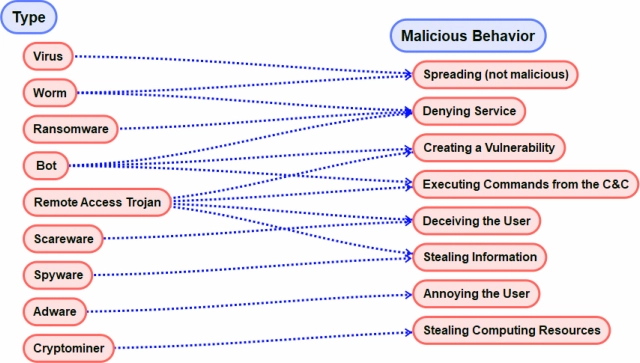
\includegraphics[width=0.7\textwidth]{obrazky/behavior.png}
	\caption{Jednotlivé typy malwaru a jejich chování, které nemusí vždy vzájemně vylučovat. Převzato z \cite{article_malware}.}
    \label{behavior}
\end{figure}
\newpage

Mezi nejběžnější typy chování patří: \cite{article_malware}
\begin{itemize}
    \item \textbf{Šíření} - S tímto chováním se setkámae nejčastěji u malwaru typu virus nebo červ. Jejich hlavním cílem je se, co nejvíce rozšířit a tím případně zahltit službu uživatele. Malware se může šířit mnoha způsoby například přes internetovou síť nebo stažením z kompromitovaných webových stránek a tak dále.
    \item \textbf{Kráděž informací} - Jedná se nejspíš o nejčastější činnost malwaru. Jedná se o čínnost, kdy malware připravuje oběti o citlivé informace, jako jsou čísla účtů, hesla, přístupové údaje za cílem zpeněžit ukradená data přímým použitím nebo jejich nelegální distribucí. Existuje několik způsobů, jak tyto informace krást, například zaznamenávání kláves (anglicky \textit{keylogger}), který zaznamenává všechny zmáčnuté klávesy \cite{data_stealing}.
    \item \textbf{Odepření služby} - K odepření služby může dojít několika způsoby. Jedná se například o zahlcení nějaké služby nebo serveru velkým množstvím falešných požadavků (k tomuto účelu se používájí \textit{botnets} \ref{botnets}). Nebo tohoto lze docílim pomocí \textit{červů}, kterří se šíří skrz počítačovou síť a tím ji můžou zahltit \cite{dos}.
    \item \textbf{Vytváření zranitelnosti} - Hlavním typem malwaru, který vytváří další zranitelnosti jsou Trojští koně. Ti po infiltraci systému vytváří nové zranitelnosti odstraněním antivirových programů, instalací zadních vrátek, změnou nastavení brány firewall.
\end{itemize}

Mezi další chování, které lze u malwaru pozorovat patří \textbf{krádež zdrojů počítaře} například na těžbu kryptoměn. Dále třeba \textbf{podvádění uživatele} k získání přístupu k soukromým datům, toto chování je běžné pro malware útočíčí na banky za cílem získat přístup k bankovním účtům a získat peníze \cite{article_malware}.

Chování je tedy nespočet a zde byly představeny pouze nejznámější a nejčastěji se vyskytující chování. Malwary patřící do stejného typu se můžou prokazovat různým chováním a nemusí mít pouze jedno chování, ale kombinace těchto chování.
%https://www.trendmicro.com/vinfo/us/security/definition/Data-Stealing-Malware
%https://www.snaptechit.com/article/the-top-4-ways-malware-is-spread-2/
%\section{Zpusoby detekce zalozene na strojovem uceni}
%https://www.ripublication.com/ijcir21/ijcirv17n1_01.pdf
%https://media.kaspersky.com/en/enterprise-security/Kaspersky-Lab-Whitepaper-Machine-Learning.pdf
%file:///home/xvenc/Downloads/preprints202209.0103.v1.pdf
%https://ieeexplore.ieee.org/abstract/document/8949524
\section{Analýza malwaru}
Pro detekci malwaru založeného na strojovém učení a jeho následného dělení je nutné porozumět dvěma základním přístupům k jeho analýze. Analýza malwaru je proces jejiž cílem je určit funkčnost, původ a možný dopad škodlivého vzorku na daný systém \cite{analysis_wiki}.

Tento proces je velice důležitý pro boj s malwarem. Pro vývoj kvalitních detekčních technik a taky pro vývoj nástrojů, které mají malware ze systému odstranit. Analýzu malware lze provádět za různými účely ať už je to za účelem pochopení, jak malware funguje
nebo pro lepší představu o rozsahu infekce a nebo za účelem zjištění následků útoku \cite{article_analysis_goat}.

Pro analýzu malwaru se používají dvě různé metody. \textbf{Statická analýza} malwaru a \textbf{dynamická analýza} malwaru. 
Jak už lze odvodit z jejího jména tak statická analýza se provádí bez spuštění malwaru. Naproti tomu dynamická analýza se provádí spuštěním malwaru v kontrolovaném prostředí, 
jako třeba ve virtualním prostředí \cite{article_analysis}.

\subsection*{Statická analýza}
Statická analýza je proces analýzy malwaru, aniž by byl skutečně spuštěn. Bývá tedy bezpečnější než analýza dynamická. Někdy se o statické analýze mluví jako o "čtení" zdrojového nebo binárního kódu za účelem
odvození chovaní malwaru. Statická analýza je aplikována na zdrojový kód a nebo pokud není zdrojový kód k dispozici (což je častější varianta) tak na binární kód. Ovšem při kompilaci zdrojového kódu na binární se nějaké informace ztratí \cite{article_analysis_goat,static_analysis}.

Pro statickou analýzu malwaru se používají různé techniky. Některé z nich jsou popsány níže \cite{malware_d_s}.
\begin{itemize}
    \item \textbf{Otisky souborů} (\textit{file fingerprint}) je jeden ze způsobů statické analýzy, který spočívá ve vypočítání kryptografického hashe (např. md5) binárního souboru za účelem jeho odlišení od jiných souborů \cite{static_analysis}.
    \item \textbf{Anti-virové skenování} (\textit{AV scanning}) je velice účínný způsob pokud je malware dobře známý, tak je vysoce pravděpodobné, že bude jedním z AV skenerů detekován. Ovšem jejich použití je časově náročné, ale někdy se stává nutností \cite{article_analysis_goat}.
    \item \textbf{Rozebraní} spíše známé pod pojmem (\textit{disassembly}) je zřejmě nejběžnější a nejspolehlivější metoda staické analýzy. Tato metoda představuje rozebrání binárního souboru pomocí speciálního nástroje, který jej převede do strojového kódu programovacího jazyka assembler. Na jehož základě lze zkontrolovat logiku programu a prozkoumat tak jeho záměr \cite{article_analysis_goat}. 
\end{itemize}

Dále se lze setkat například s metodami založenými na extrakcí řetězců nebo na Kontrola formátu souboru.

Výhodou statuické analýzy je, že umožnuje vysoce komplexní analýzu, jak zdrojového kódu tak binárního souboru. Navíc je bezpečnejší než dynamická analýza a nehrozí tedy nechtěná infekce uživatelského počítače.
Ovšem hlavní nevýhodou statické analýzy je její časová náročnost, těžkopádnost a proto jsou pro ni vyžadovány odborné znalosti \cite{article_analysis_goat}.

\newpage
\subsection*{Dynamická analýza} \label{dynamic}
Spuštění malware vzorku v kontrolovaném prostředí za účelem sledování a analýzy jeho škodlivého chování se nazývá dynamická analýza.
Narozdíl tedy od statické analýzy je zde chování, vlastonsti a záměry malwaru sledováno během jeho spuštění.
Díky tomu lze snadno zjistit skutečné chování programu. Další významnou výhodou je, že lze automatizovat, což umožňuje analýzu ve velkém měřítku a taky značně rychlejší než analýza statická.

Ovšem nevýhodou je takzvaný \uv{spící kód}. To znamená, že na rozdíl od statické analýzy dynamická analýza obvykle sleduje pouze jednu cestu provádění, a proto se někdy projevu
neúplným pokrytím kódu \cite{article_analysis_goat}. Další nevýhodou je, že malwary jsou stále chytřejší a vědí, že se malware je spouštěn ve virtuálním prostřední, a proto záměrně zůstávají neaktivní dokud nejsou splněny určité podmínky. Takovýmto příkladem je třeba malware \textit{Loki} \cite{malware_analysis}.

Během tohoto druhu analýzy,je možné zjistit všechny atributy chování, jako jsou otevřené soubory, vytvořené mutexy, s jakými servery malware komunikoval a jaké pakety byly odeslány a mnoho dalšího.
Aby nedošlo k poškození uživatelského počítače, tak jsou vzorky malwaru spouštěny ve virtualních prostředích (častěji označovanými jako \textit{sandbox} prostředí nebo jen \textit{sandboxy}) \cite{malware_analysis}. Sandboxy slouží jako bezpečnostní pojistka, aby
nebylo nutné malware spouštět na svém počítači a tím ho vystavit nebezpečí. Ovšem drobnou nevýhodou sandbox prostředí je, že se dosažené výsledky analýzy mohou na různých operačních systémech lišit.

Lze rozlišit dva základní přístupy dynamické analýzy a to jsou:
\begin{itemize}
    \item \textbf{Analýza rozdílu mezi body} - Analýza daného vzorku je prováděna po určitou dobu. Poté jsou zanalyzovány změny, které v systému nastali oproti původnímu stavu systému \cite{article_analysis_goat}.
    \item \textbf{Pozorování chování během běhu} - V tomto případě je monitorována a analyzována škodlivé aktivity, které při spuštění malwaru nastanou pomocí specializovaných nástrojů \cite{article_analysis_goat}. 
\end{itemize}

\subsection*{Závěr}
Analýza malwaru je velice důležitá činnost, která slouží k pochopení, jak malware funguje a jak nám může uškodit. Tím, že víme, jak malware funguje se proti němu lze účiněji bránit a také zvyšujeme šanci, že se nám ho 
podaří zachytit dřive než napáchá nějaké škody. 

V této sekci byly deta představeny dva přístupy analýzy, které jsou velice odlišné, ale obě se v dnešní době hojně používají.

%https://www.researchgate.net/publication/276967529_Implementation_of_Malware_Analysis_using_Static_and_Dynamic_Analysis_Method
%http://www.differencebetween.net/technology/difference-between-static-malware-analysis-and-dynamic-malware-analysis/
%https://hackercombat.com/static-malware-analysis-vs-dynamic-malware-analysis/
%https://web.archive.org/web/20160418151823/http://www.ijarcsse.com/docs/papers/Volume_3/4_April2013/V3I4-0371.pdf
%https://www.crowdstrike.com/cybersecurity-101/malware/malware-analysis/
%https://dl.acm.org/doi/pdf/10.1145/3329786
%file:///home/xvenc/Downloads/Basic%20Static%20Malware%20Analysis%20using%20open%20source%20tools.%20B.%20Jaya%20Prasad,%20Haritha%20Annangi%20&%20Krishna%20Sastry%20Pendyala.pdf

\chapter{Automatické vytváření datových sad} \label{3.chap}
%Proč jsou datasety důležité, popsat můj nástroj na tvorbu datasetů. Co je jeho výstupem a jak funguje. Popsat co jsou pcapy, co se vyskytuje v reportech, co je to sandbox prostredi. proc zrovna tento sandbox, zminit i jine.
%Jedna se o jednudochou pipeline a je na obrazku, jednotlive vstupy a vystupy casti jsou popsany v nasledujicich podkapitolach.

Podstatnou a velice důležitou částí této práce je výběr a tvorba vhodných datových sad (z anglického \textit{datasets}).
Protože v této práci je využito stojového učení, je na vytvoření žádoucí datové sady kladen velký důraz. 
S daty totiž souvisí důveryhodnost dosažených výsledků.
Proto byl pro tvorbu žádoucích datových sad vytvořen nástroj, který bude v následující kapitole představen. 

Tato kapitola tedy pojednává o postupu vytváření datových sad. Nejprve je tento proces zjednodušeně popsán.
Poté jsou zde detailně popsány jednotlivé části tohoto procesu popsány a co je jejich vstupem a výstupem.
A nakonec jsou představeny technologie a programovací jazyk, který byl pro toto vytváření zvolen. 

%Tato kapitola tedy pojednává o vybraném programovacím jazyce a knihovnách používaných pro danou úlohu. 
%Poté je popsána obecný proces vytváření těchto datových sad. A nakonec jsou zde popsány jednotlivé části tohoto procesu a 
%jak vypadá skutečný výstup programu.

\section{Postup vytváření datových sad}
Zjednodušený proces tvorby datasetů lze vidět na obrázku \ref{pipeline}, kde je znázorněno jednoduché schéma procesu, jak vytvořený nástroj pracuje. 

Nejprve tedy nástroj stáhne odpovídající počet malware vzorků z volně dostupného databázového serveru. Tyto vzorky jsou pak poslány na server, kde je provedena dynamická analýza.
Pro každý vzorek se provedou dvě analýzy každá na jiném referenčním stroji.
Po dokončení analýzy vzorků jsou ke každému vzorku staženy dva soubory se zachycenou síťovou kumunikací malwaru v podobě \textit{pcap} souborů a ješte zpráva shrnující analýzu daného vzorku.
Každá část tohoto procesu bude detailně popsáno v následujících sekcích, kde budou uvedy i příklady výstupů a výstupů dílčích částí.\\

\begin{figure}[h]
	\centering
        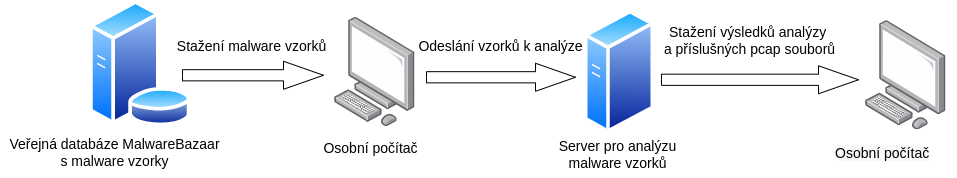
\includegraphics[width=0.8\textwidth]{obrazky/pipeline.png}
	\caption{Proces vytváření datasetů}
    \label{pipeline}
\end{figure}

\section{Stahování malware vzorků}
Prvním krokem je stažení dostatečného počtu malware vzorků pro jednotlivé malware rodiny. Jediným vstupem do toho nástroje od uživatele je tedy pouze textový soubor, který obsahuje
jména rodin. Všechny vzorky jsou stahovány z veřejně dostupné databaze \textit{MalwareBazaar}\footnote{\href{https://bazaar.abuse.ch/}{https://bazaar.abuse.ch/}}. Tato databáze je 
bezplatná a lze stahovat neomezený počet vzorků na rozdíl od jiných databazí jako například \textit{VirusTotal}\footnote{\href{https://www.virustotal.com/gui/home/upload}{https://www.virustotal.com/}}.

Názvy rodin malware musí být stejné jako je specifikuje \textit{MalwareBazaar}, aby nedošlo k nějaké záměně s jiným druhem malwaru. Každý vzorek je poté stažen, jako zaheslovaný zip soubor, aby omylem nedošlo k 
jeho něchtěnému spuštění. Vzorky jsou uloženy podle rodin, aby z důvodu jednoduššího vyhledávání. Jediným omezením je maximalní počet malware vzorků stažených pro jednu rodinu, který činí 1000 vzorků.

\section{Analýza vzorků}
%popsat pcapy, jak probíha analyza, sandboxy
V dalším kroku je nutné veškeré stažené vzorky analyzovat. Každá analýza je prováděna v sandbox prostředení, aby nedošlo k žádnému poškození uživatelského počítače.
Použitým sandbox prostředím pro analýzu je nástroj zvaný \textit{Triage}\footnote{\href{https://tria.ge/dashboard}{https://tria.ge/dashboard}}. Tento nástroj byl vybrán kvůli jeho škálovatelnosti a rychlosti, 
ale především kvůli jeho komplexnímu API rozhraní.

Pro každý vzorek jsou provedeny dvě automatické dynamické analýzy \ref{dynamic} ve dvou různých virtuálních prostředích a jedna statická analýza (ta ovšem není pro tuhle práci tak důležítá, proto se jí dále nebudeme zabývat). 

Celkový proces od nahrání vzorku až po vytoření výsledné zprávy lze vidět na obrázku \ref{Analysis_diagram}. Z něj je patrné, že probíhájí dvě oddělené analýzy. První analýza je prováděno na virtuálním stroji, kde beží 
systém Windows 7 a druhá analýza je prováděna v prostředí se systémem Windows 10.

\begin{figure}[h]
	\centering
        \includegraphics[width=0.6\textwidth]{obrazky/diagram.pdf}
	\caption{Proces analýzy malware vzorků}
    \label{Analysis_diagram}
\end{figure}

Poté, co je vzorek odeslán k analýze, tak je nejprve naplánovaná jeho statická analýza. Po skončení této analýzy je vzorek odeslán k dynamické analýze. Každá analýza se sestáva z extrakce malware vzorku, ze zip archivu. A jeho následného spuštění v čistém prostředí. Poté je zaznamenávána veškerá síťová komunikace a také veškerá aktivita, ke které dojde.
Z obou analýz je pak vygenerována výsledná zpráva.
\section{Výstup programu}
% Popsat pcapy co je v report souborech a k cemu jsou pcapy asi
% konecny vystup programu, rolozeni struktury
%Jak je možné vidět na obrázku \ref{Analysis_diagram}, tak výstupem, který lze ze sandboxu dostat jsou souhrné výsledky analýzy. Tyto výsledky představují soubor (zpráva, anglicky \textit{report}), který popisuje chování malwaru, 
Jak je možné vidět na obrázku \ref{Analysis_diagram}, tak výstupem po skončení dynamické analýzy jsou různé soubory (nebo-li zprávy, anglicky \textit{reports}). Pro účel téhle práce jsou však důležité pouze dva druhy těchto souborů.

Prvním souborem, který je pro tuhle práci relevantní, je soubor obsahující výstup dynamické analýzy. Triage sandbox poskytuje výsledek této analýzy v několika různých formátech jako je třeba XML, JSON či PDF (výstup reportu, který je pak převeden do formátu PDF lze vidět na obrázku ...).
Formát PDF není vhodný z důvodů dalšího zpracování, které bude v následujících fázích potřebné. Nelze z něj jednodušše programově vytáhnout informace. Proto je výsledek analýzy stažen ve formátu JSON.

Mezi významné informace, které lze z toho souboru vyčíst, patří název malware rodiny a krátky popis této rodiny malware. Dále potom ndikátory kompromitace (\texttt{Indicators of Compromise}, zkráceně IoC), 
jsou to tedy hlavně IP adresy a domény, na které se malware snažil připojit a vést jejich prostřednictvím útok. Dále poté může obsahovat navštívené webové stránky a mnoho dalších informací.

\begin{figure}[h]
	\centering
        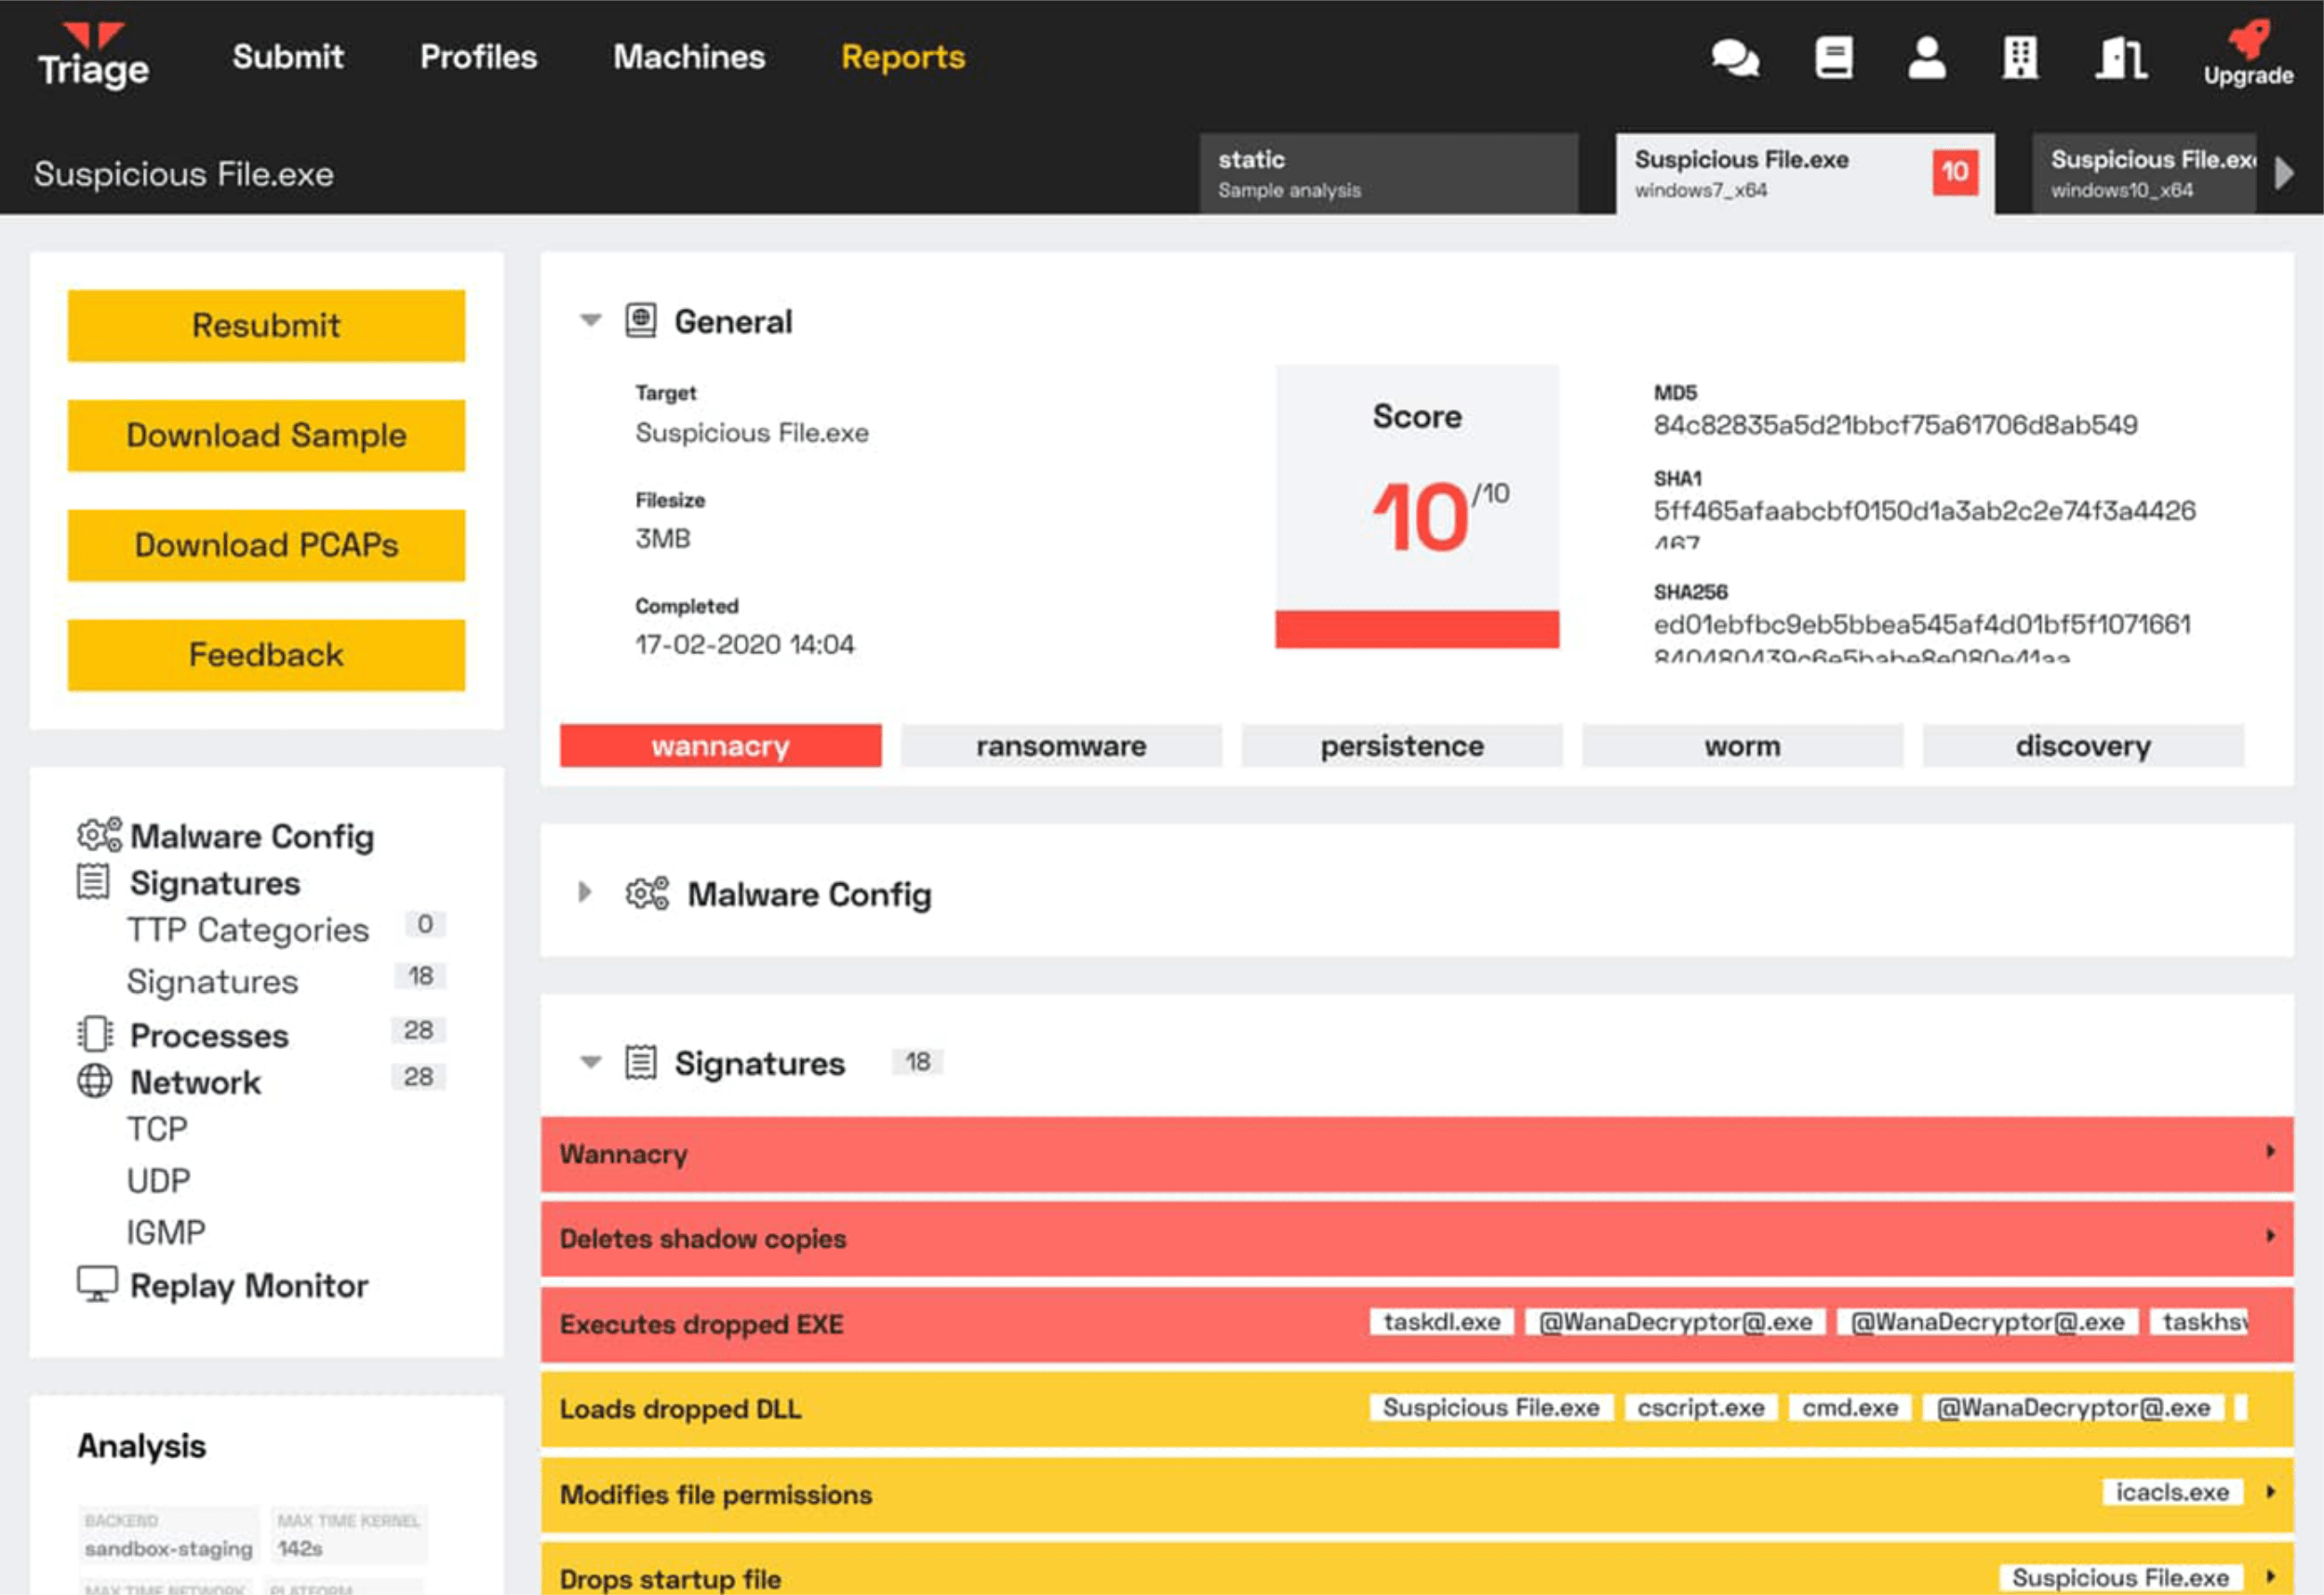
\includegraphics[width=0.7\textwidth]{obrazky/3-triage-report.png}
	\caption{Snímek obrazovky s výsledky z dynamické analýzy. Převzato z \cite{hatching}.}
    \label{Report_image}
\end{figure}

Druhým typem souboru, který je zásadním pro další zpracování jsou soubory typu \texttt{PCAP}. Pro každý malware vzorek jsou staženy dva PCAP soubory.
Tyto soubory obsahují zachycenou síťovou komunikaci ve formě paketů. Tyto soubory lze analyzovat pomocí nástroje \textit{Wireshark}\footnote{\href{https://www.wireshark.org/}{https://www.wireshark.org/}}, 
kde si lze vyfiltrovat komunikaci dle potřeby.

\newpage
\section{Využité technologie}

Veškeré skripty jsou napsány v programovacím jazyce \textbf{Python}. Tento jazyk byl zvolen hned z několika důvodů.
Především ale kvůli jeho jednoduchosti a známosti. Dále taky kvůli knihovnám pro práci s HTTP a posíláním dat po síti.
Velkou výhodou byla také implemetace oficiálního API (aplikačního webového rozhraní z anglického \textit{Application Programming Interface}) klienta pro webové rozhraní 
\texttt{tria.ge}\footnote{\href{https://tria.ge/dashboard}{https://tria.ge/dashboard}}. 
Hlavní využívanou knihovnou je tedy knihovna \textbf{tiage}. Dále se hojně využívá knihovna \textbf{requests} \footnote{\href{https://requests.readthedocs.io/en/latest/}{https://requests.readthedocs.io/en/latest/}}
pro posílaní HTTP požadavků a zpracování jejich odpovědí.

\subsection*{Triage}
Triage je knihovna sloužící ke komunikaci s aplikačním webovým rozhraním Hatching Triage. Tato knihovna usnadňuje práci s analýzou malware vzorků.
Její hlavní použití je tedy odesílaní vzorků k analýze a následné stáhnutí statických výsledků této analýzy a souborů se zachycenou síťovou komunikací v 
podobě paketů, nebo-li souborů s příponou \textit{.pcap}. Hlavní výhodou této knihovny je jednoduchá komunikace s API rozhraním a možnost extrakce všech důležitých
informací z analýzy.

\subsection*{Requests}
Requests je jednoduchá, ale efektivní knihovna pro práci s HTTP/1.1 požadavky a pro spracování odpovědí. Je zde podpora všech typů požadvků, jako jsou
třeba GET, POST, PUT, DELETE a mnoho dalších. Pro potřeby této práce byly použity pouze požadavky typu GET a POST. Dále byly taky využity možnosti
pro spracování odpovědi, ověření zda je spojení stále aktivní a nakonec samotné vytažení a uložení dat.\\ 

Mezi další knihovny, které byly v jisté malé míře použity patří:
\begin{itemize}
    \item Knihovna \textbf{csv}\footnote{\href{https://docs.python.org/3/library/csv.html}{https://docs.python.org/3/library/csv.html}}\\Pro usnadění práce s vytvořenými logovacími soubory.
    \item Knihovna \textbf{pathlib}\footnote{\href{https://docs.python.org/3/library/pathlib.html}{https://docs.python.org/3/library/pathlib.html}}\\Pro vytváření vnořených adresářových struktur a ověřování existence adresářů.
    \item Knihovna \textbf{json}\footnote{\href{https://docs.python.org/3/library/json.html}{https://docs.python.org/3/library/json.html}}\\Slouží pro k převodu slovníků na formát JSON a lepší extrakci informací z tohoto formátu.
\end{itemize}



%Cca 4 stranek
    
\chapter{Závěr}
Cílem dosavadní práce bylo porovnání dostupných datových sad, které obsahují malware komunikaci. Dála bylo zapotřebí vybrat vhodné prostředí pro 
pro tvorbu vlastních datových sad. A nakonec bylo zapotřebí vytvoření automatického nástroje na tvorbu nových datasetů.

Nástroj se zatím ukazuje jako funkční a dostatečný pro budoucí potřeby této práce. A na získávání vetšího počtu malware vzorků je i poměrně efektivní.

Následujícími kroky v práci bude extrakce významných prvků jak ze souborů PCAP tak z výsledků statické a dynamické analýzy.
Dále následuje implementace vhodných metod pro detekci malware na základě strojového učení. Bude se jednat o metody založené na rozhodovacích stromech.
Nakonec je bude potřeba tyto metody porovnat a zhodnotit výsledky celkové práce pro vytvořené datasety.


%===============================================================================

% Pro kompilaci po částech (viz projekt.tex) nutno odkomentovat
%\end{document}
